\documentclass[a4paper,12pt]{extarticle}

\usepackage[left=2.5cm,right=1.0cm,top=2.0cm,bottom=2.0cm]{geometry}
\usepackage[T1,T2A]{fontenc}
\usepackage[utf8]{inputenc}
\usepackage[main=english,russian]{babel}
\usepackage{amsmath}
\usepackage{amssymb}
\usepackage{booktabs}
\usepackage{array}
\usepackage{float}
\usepackage{graphicx}
\usepackage{indentfirst}
\usepackage{setspace}
\usepackage{tikz}
\usepackage{url}
\usepackage[
backend=biber,
style=numeric,
sorting=none,
maxbibnames=99
]{biblatex}
\usepackage[colorlinks,citecolor=blue,linkcolor=blue,urlcolor=blue]{hyperref}

\addbibresource{refs.bib}

\usetikzlibrary{arrows.meta,positioning,shapes.geometric}
\graphicspath{{figures/report/}{experiments/window_ablation/figures/}{experiments/horizon_ablation/figures/}{experiments/threshold_event_tuning/figures/}{experiments/classical_baselines/figures/}}

\setlength{\parindent}{1.25cm}
\onehalfspacing

\usepackage{chngcntr}
\counterwithin{table}{section}
\counterwithin{figure}{section}

\begin{document}

\begin{titlepage}
\newpage

{\setstretch{1.0}
\begin{center}
NATIONAL RESEARCH UNIVERSITY\\
HIGHER SCHOOL OF ECONOMICS
\\
\bigskip
Faculty of Computer Science\\
Bachelor's Program ``Data Science and Business Analytics''
\end{center}
}

\vspace{3em}

\begin{center}
{\bf Research Project Report on the Topic:}\\
\vspace{1em}
{\bf Behavioral Detection of Cryptominers Using System Workload Data}
\end{center}

\vspace{3em}

{\bf Submitted by the Student: \vspace{2mm}}

{\setstretch{1.1}
\begin{tabular}{l@{\hskip 1.5cm}l}
group \foreignlanguage{russian}{БПАД} 246, 2nd year of study &
Mandrykin Andrei \\
\end{tabular}}

\vspace{2em}

{\bf Approved by the Project Supervisor: \vspace{2mm}}

{\setstretch{1.1}
\begin{tabular}{l}
Petr Grinberg\\
Visiting Lecturer\\
Faculty of Computer Science, HSE University
\end{tabular}}

\vspace{\fill}

\begin{center}
Moscow 2026
\end{center}

\end{titlepage}

\newpage
\setcounter{page}{2}

{
\hypersetup{linkcolor=black}
\tableofcontents
}

\newpage
\section*{Annotation}
\addcontentsline{toc}{section}{Annotation}

Cryptomining malware covertly uses a victim's computational resources and is difficult to detect by file signatures because malware samples can be obfuscated, modified, or executed only in memory. This course project develops and evaluates a host-based behavioral detector that uses only system workload telemetry. The proposed method trains a Temporal Convolutional Network on normal telemetry in a self-supervised forecasting setting and treats large future-prediction errors as anomaly evidence. The implemented pipeline collects and preprocesses telemetry, constructs temporal windows, trains the model, scores infected and mixed scenarios, and automatically generates report tables and figures. The final configuration uses 30-second input windows, a 10-second prediction horizon, and a 10-second stride. On five mixed normal-infected scenarios the detector achieved mean precision of 1.0000, mean recall of 0.9754, mean F1-score of 0.9872, and zero false positives at the selected threshold. The results show that workload-based anomaly detection is a practical complementary approach to signature-based cryptominer detection.

\section*{\foreignlanguage{russian}{Аннотация}}
\addcontentsline{toc}{section}{Аннотация}
\foreignlanguage{russian}{
Вредоносное программное обеспечение для криптомайнинга скрытно использует вычислительные ресурсы зараженной системы и может обходить сигнатурные методы обнаружения за счет обфускации, модификации исполняемых файлов или запуска без устойчивых файловых индикаторов. В данной курсовой работе разработан и экспериментально проверен поведенческий детектор, использующий только телеметрию системной нагрузки. Предложенный метод обучает Temporal Convolutional Network на нормальном поведении системы в режиме самоконтролируемого прогнозирования, а большие ошибки прогноза использует как признак аномалии. Реализованный пайплайн выполняет предобработку телеметрии, построение временных окон, обучение модели, оценку зараженных и смешанных сценариев, а также автоматическую генерацию таблиц и графиков отчета. Финальная конфигурация использует окно длиной 30 секунд, горизонт прогноза 10 секунд и шаг 10 секунд. На пяти смешанных сценариях нормальной и зараженной активности получены средние precision 1.0000, recall 0.9754, F1-score 0.9872 и нулевая доля ложных срабатываний. Результаты показывают, что анализ системной нагрузки может служить практичным дополнением к сигнатурному обнаружению криптомайнеров.
}

\section*{Keywords}
\addcontentsline{toc}{section}{Keywords}
Cryptomining malware, cryptojacking, behavioral detection, system workload, anomaly detection, Temporal Convolutional Network, time-series forecasting, cybersecurity.

\newpage
\section{Introduction}
\label{sec:introduction}

Cryptomining malware, also called cryptojacking malware, is a class of malicious software that uses a victim's CPU or GPU resources to mine cryptocurrency for an attacker \cite{darabian2020cryptomining,almurshid2024holistic}. Unlike destructive malware, a cryptominer is economically useful to the attacker only while it remains active, so it is usually designed to operate quietly for long periods of time. This causes persistent performance degradation, increased power consumption, hardware wear, and unexpected network activity while leaving the user with few obvious symptoms.

Classical malware detection relies heavily on signatures, known indicators of compromise, static code features, and manually defined rules. These methods remain useful against known samples, but they are fragile when a malicious program is repacked, obfuscated, throttled, or otherwise modified. Cryptominers are especially suitable for such evasion because their malicious payload can be small while the actual mining process may look like an ordinary resource-intensive computation.

The main idea of this project is to detect cryptomining through its operational effect rather than through the executable file itself. Even if a miner hides its code, it still needs to consume CPU or GPU cycles, memory, process resources, and network bandwidth \cite{darabian2020cryptomining,almurshid2024holistic}. These signals can be represented as multivariate time series and analyzed with deep learning. The project therefore focuses on host-based workload telemetry: CPU and RAM utilization, disk and network throughput, and statistics of the most resource-consuming processes.

The objective of the work is to build and evaluate a proof-of-concept behavioral cryptominer detector that uses system workload data only. The detector must not rely on executable hashes, static code analysis, mining pool blacklists, or signatures. The implemented solution trains a forecasting model on normal behavior and marks sustained high prediction error as anomalous.

The following research questions are addressed:
\begin{itemize}
    \item Can cryptomining activity be detected using only host workload telemetry?
    \item Which workload features contribute most to the anomaly score?
    \item How sensitive is the detector to the temporal window length, prediction horizon, and event threshold?
    \item How does the proposed deep learning detector compare with classical anomaly detection baselines?
\end{itemize}

The main contribution of this work is an end-to-end experimental pipeline for workload-based cryptominer detection. It includes data preparation, temporal window generation, a Temporal Convolutional Network (TCN) forecasting model, anomaly scoring, event-level postprocessing, evaluation on infected-only and mixed scenarios, ablation experiments, baseline comparison, and automatic generation of tables and figures for analysis. The final model reaches mean F1-score 0.9872 on the mixed scenarios used in the project while maintaining zero false positives at the selected threshold.

\newpage
\section{Related Work}
\label{sec:related}

Malware detection has traditionally been based on signature matching, static analysis, heuristic rules, and known behavioral indicators. These approaches are practical and efficient for known threats, but they often struggle with malware variants that are obfuscated or packed. Surveys of deep learning malware detection emphasize that static signatures alone are insufficient against rapidly changing malware families and that behavioral information is important for detecting unknown or modified samples \cite{redhu2024deep}.

Cryptomining malware is a specific subclass of malware whose goal is resource theft rather than direct data destruction. Darabian et al. \cite{darabian2020cryptomining} proposed a deep learning approach for cryptomining malware detection using both static opcode sequences and dynamic system-call traces. Their work demonstrates that cryptominers have learnable runtime behavior, but the features are still closely tied to executable-level analysis and sandbox instrumentation. In contrast, the present project uses only coarse host workload telemetry, which is easier to collect continuously on an endpoint and does not require inspecting the executable.

Almurshid et al. \cite{almurshid2024holistic} proposed a holistic intelligent cryptojacking detection system that combines static analysis, dynamic analysis, and deep learning. This line of work confirms the importance of cryptojacking-specific detection but also illustrates the complexity of systems that require several analysis channels. The method developed in this course project is narrower but lighter: it evaluates whether a detector can work from system load measurements alone.

Machine learning methods for anomaly detection are often used when labeled malicious data are limited or when new attack variants are expected \cite{redhu2024deep}. Classical one-class methods such as One-Class SVM and Isolation Forest can model normal behavior without requiring malicious examples. However, they usually treat each window as a fixed feature vector and may not capture temporal structure as directly as sequence models.

Temporal Convolutional Networks are a natural fit for time-series modeling. Bai, Kolter, and Koltun \cite{bai2018tcn} showed that causal and dilated convolutional architectures are strong general-purpose sequence models and can provide long effective memory with efficient parallel computation. This project uses a TCN as a forecasting model: it learns normal short-term workload dynamics and uses deviations between predicted and observed future telemetry as anomaly evidence.

The project is positioned between host-based behavioral malware detection and time-series anomaly detection \cite{darabian2020cryptomining,redhu2024deep}. Its practical novelty is not a new neural network architecture, but the application and evaluation of TCN forecasting \cite{bai2018tcn} to cryptominer detection using lightweight endpoint workload metrics, together with a reproducible pipeline and a detailed empirical analysis of thresholds, temporal parameters, and feature importance.

\newpage
\section{Data and Preprocessing}
\label{sec:data}

\subsection{Data collection environment}

Telemetry data were collected using a controlled experimental environment designed to capture both normal and infected system behavior under realistic workload conditions.

\subsubsection{Host System}

The experiments were conducted on a host machine with the following hardware configuration:

\begin{itemize}
    \item Operating system: Windows 11 home
    \item Processor (CPU): AMD Ryzen 9 5900X 12-Core Processor 
    \item Graphics processing unit (GPU): Nvidia GeForce RTX 3070
    \item System memory (RAM): 32,0 GB
    \item Storage type: SSD/HDD
\end{itemize}

\subsubsection{Virtual Machine Configuration}

Malware execution was isolated inside a virtualized environment to ensure safe collection of infected telemetry while preventing interference with the host operating system.

The virtual machine configuration was the following:

\begin{itemize}
    \item Virtualization software: Oracle VirtualBox
    \item Guest operating system: Windows 11 home
    \item Allocated CPU cores: 12
    \item Allocated RAM: 20192 MB
    \item Allocated storage: 80 GB
    \item Network configuration: NAT
    \item VPN enabled: V2rayN
\end{itemize}

\subsubsection{Telemetry Collection Pipeline}

System telemetry was collected using a custom Python-based telemetry collector developed specifically for this work. The collector recorded workload statistics at a sampling frequency of 1 Hz = 1s.

For process-level monitoring, the collector tracked the $K=5$ most computationally active processes and extracted behavioral features including CPU utilization, memory consumption, thread count, and process lifetime.

Missing values and timestamp irregularities were corrected during preprocessing by resampling telemetry streams to an exact 1 Hz temporal grid.

\subsubsection{Software Environment}

The deep learning pipeline was implemented using Python.

The software stack included:

\begin{itemize}
    \item Python 
    \item PyTorch 
    \item NumPy
    \item Pandas
    \item Psutil
    \item Matplotlib
    \item scikit-learn
\end{itemize}

Model training and evaluation were performed on AMD Ryzen 9 5900X 12-Core Processor/Nvidia GeForce RTX 3070 (CPU / GPU specification).

\subsection{Telemetry structure}

The dataset consists of cleaned CSV telemetry files sampled at 1 Hz. Each row describes the system state at one second. The feature vector contains 26 numerical workload indicators after removing the timestamp column. The feature groups are:
\begin{itemize}
    \item global CPU and RAM utilization;
    \item network input and output throughput;
    \item disk read and write throughput;
    \item CPU, memory, thread count, and process age for the top resource-consuming processes.
\end{itemize}

The cleaned dataset used in the final pipeline contains seven normal files, five infected-only files, and five mixed files. One normal file is reserved as a holdout background for mixed scenarios and is not used for fitting the normal baseline or the validation threshold. The mixed scenarios are constructed as a concatenation of normal activity, a fixed infected interval, and normal activity after the infected interval.

GPU columns were deliberately excluded from the final feature set. During dataset inspection, infected files were found to contain GPU columns filled with constant zeros because of collection limitations. Keeping these fields would allow the detector to exploit a data-collection artifact rather than cryptomining behavior. Therefore, all columns with the \texttt{gpu\_} prefix are removed before dataset construction, training, scoring, and feature-importance analysis.

\subsection{Data Collection Scenarios}

The telemetry dataset was collected under multiple operating conditions to capture diverse system behavior patterns and improve model generalization. The collected scenarios were divided into two groups: legitimate system activity and malware-infected activity.

\subsubsection{Normal Activity Scenarios}

Normal telemetry was collected during everyday computer usage intended to represent legitimate user behavior. Multiple workload categories were included to increase behavioral diversity.

The following scenarios were recorded:

\begin{itemize}
    \item Idle system operation
    \item Idle operation with VPN enabled
    \item Web browsing activity
    \item Spotify audio playback
    \item Gaming workloads (Overwatch)
    \item Video streaming workloads
\end{itemize}

Browser-related workloads included realistic user interaction patterns such as page navigation, video playback, and media consumption.

The following websites were used during browser-based data collection:

\begin{itemize}
    \item YouTube
    \item Twitch
    \item Spotify Web Player
    \item General web browsing sessions
\end{itemize}

The objective was to expose the model to realistic variations in CPU utilization, memory consumption, network throughput, disk activity, and GPU workload.

\subsubsection{Malware-Infected Scenarios}

Telemetry corresponding to infected system behavior was collected inside the isolated virtual machine environment described in Section 3.1.

Cryptomining malware samples were executed while simultaneously generating legitimate foreground activity to simulate realistic user behavior during infection.

Background workloads during infected data collection included:

\begin{itemize}
    \item Browser activity  
    \item Video playback
    \item Audio playback
    \item Gaming-related workloads
    \item Idle periods
\end{itemize}

Browser activity was collected while using these websites (opened tabs of youtube.com, amazon.com, netflix.com, spotify.com, twitch.com, yandex.ru, x.com).

This design aimed to prevent the anomaly detection model from relying solely on high CPU utilization as an infection indicator and instead encourage learning richer behavioral patterns.

\subsubsection{Malware Acquisition}

Malware samples were obtained from publicly available malware repositories on malwarebazaar.com.

Samples were selected based on cryptomining-related characteristics and Windows platform compatibility.

The evaluated malware families included:

\begin{itemize}
    \item XMRig-based cryptominers
    \item SilentCryptoMiner
    \item Additional Monero-oriented mining malware variants
\end{itemize}

Malware execution was performed exclusively within isolated virtual environments to minimize safety risks.

\subsubsection{Mixed Evaluation Scenarios}

In addition to purely normal and purely infected telemetry, mixed scenarios were constructed to evaluate the ability of the model to detect behavioral transitions.

Mixed recordings combined normal and infected segments into a single telemetry sequence.

The mixed scenario construction followed the pattern:

\begin{equation}
Normal \rightarrow Infected \rightarrow Normal
\end{equation}

This evaluation setup was designed to measure detection latency and transition detection capability under conditions closer to real-world deployment.

\subsection{Temporal window construction}

The final model configuration is defined in \texttt{project\_config.py}: input length $T=30$ seconds, prediction horizon $H=10$ seconds, and stride $S=10$ seconds. For a normalized telemetry matrix $X \in \mathbb{R}^{N \times D}$, where $D=26$, each sample consists of a past window and a future target:
\begin{equation}
    X_{\mathrm{past}}^{(i)} = X_{iS:iS+T-1}, \qquad
    Y_{\mathrm{future}}^{(i)} = X_{iS+T:iS+T+H-1}.
    \label{eq:window}
\end{equation}
The model receives $X_{\mathrm{past}}^{(i)}$ and predicts $Y_{\mathrm{future}}^{(i)}$.

Training and validation windows are constructed only from normal telemetry. In the final dataset there are 2360 training windows and 590 validation windows. Normalization parameters are fitted on the training split and then applied to training, validation, infected, and mixed data.

\begin{figure}[H]
\centering
\begin{tikzpicture}[
node distance=1.6cm,
box/.style={rectangle, rounded corners, draw, align=center, minimum width=3.1cm, minimum height=0.9cm},
arrow/.style={-{Latex[length=3mm]}, thick}
]
\node[box] (raw) {Raw telemetry\\CSV files};
\node[box, right=of raw] (clean) {Cleaning and\\1 Hz alignment};
\node[box, right=of clean] (windows) {Temporal\\windows};
\node[box, below=of windows] (train) {TCN training\\on normal data};
\node[box, left=of train] (score) {Forecasting error\\and anomaly score};
\node[box, left=of score] (report) {Metrics, tables,\\figures};
\draw[arrow] (raw) -- (clean);
\draw[arrow] (clean) -- (windows);
\draw[arrow] (windows) -- (train);
\draw[arrow] (train) -- (score);
\draw[arrow] (score) -- (report);
\end{tikzpicture}
\caption{Implemented experimental pipeline from telemetry files to report artifacts.}
\label{fig:pipeline}
\end{figure}

Figure~\ref{fig:pipeline} summarizes the implemented pipeline. The same scripts are used to generate model checkpoints, score files, JSON evaluation results, CSV/Markdown tables, and plots.

\begin{figure}[htbp]
    \centering
    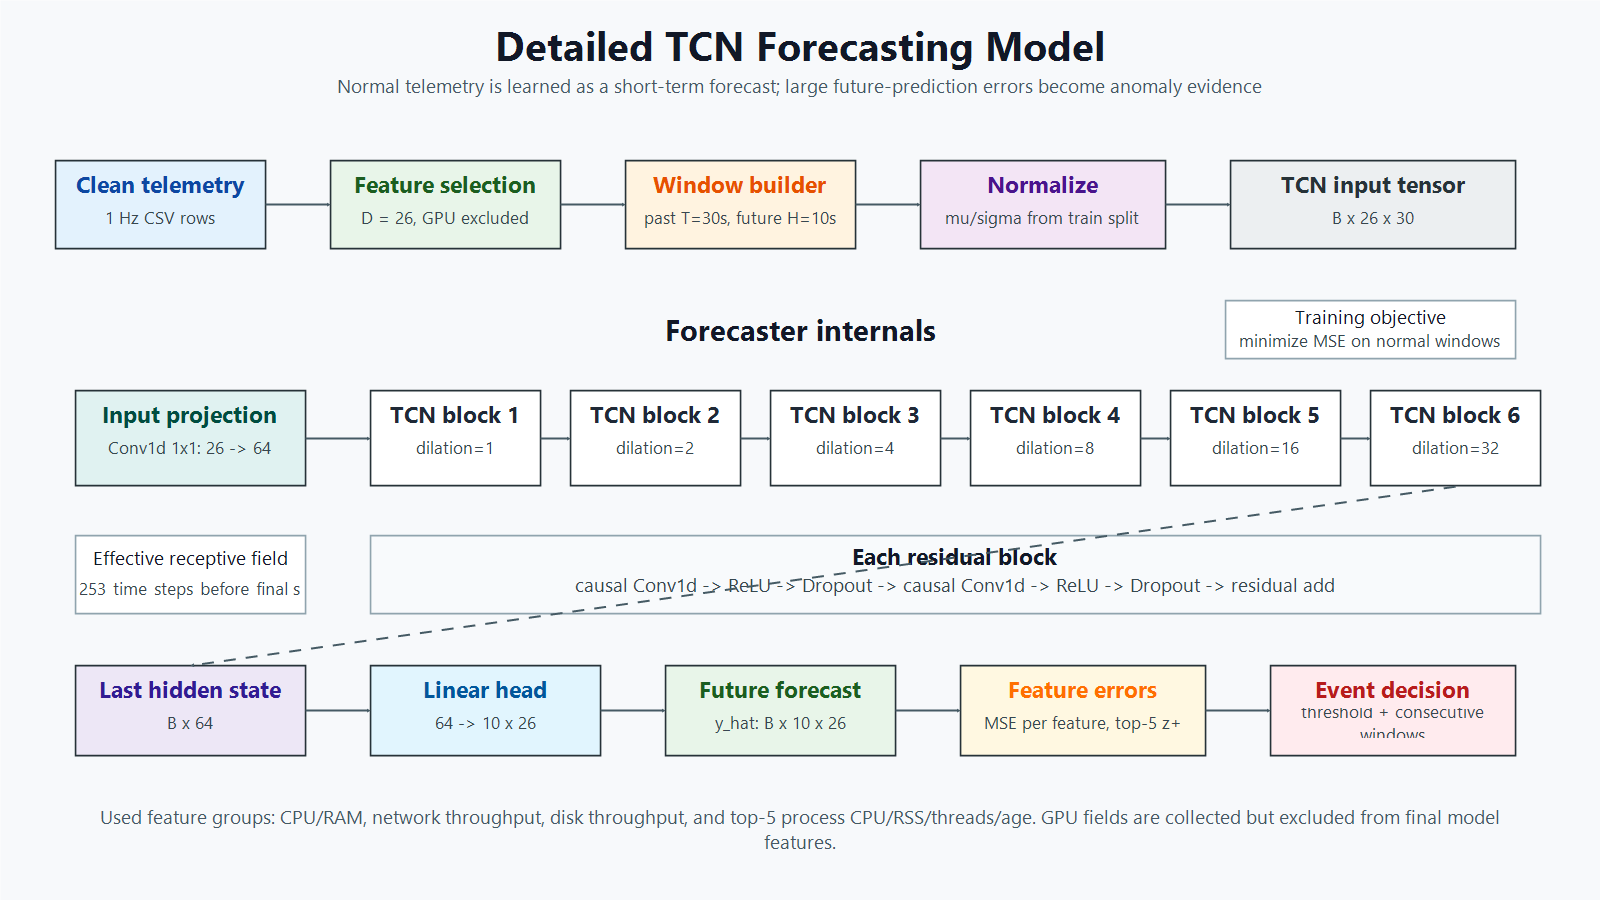
\includegraphics[width=\textwidth]{tcn_model_detailed_visualization.png}
    \caption{Detailed architecture of the TCN forecasting model used for anomaly detection. The diagram shows the telemetry preprocessing pipeline, input tensor construction, TCN residual blocks with increasing dilation rates, future forecasting head, feature error computation, and final event decision stage.}
    \label{fig:tcn_model_detailed_visualization}
\end{figure}

Figure~\ref{fig:tcn_model_detailed_visualization} illustrates the proposed TCN forecasting pipeline. Normal telemetry is transformed into input windows, passed through dilated residual TCN blocks, and used to forecast future feature values. Large forecasting errors are then interpreted as evidence of anomalous behavior.

\section{Method}
\label{sec:method}

\subsection{Forecasting model}

The detector uses a Temporal Convolutional Network \cite{bai2018tcn}. The model first projects the $D=26$ input features into a hidden representation with a one-dimensional convolution. This is followed by residual TCN blocks with causal dilated convolutions. Causality ensures that predictions depend only on past samples, while dilation increases the receptive field without requiring a very deep network. The final linear layer maps the last hidden state to a flattened $H \times D$ future prediction.

The model is trained with mean squared error:
\begin{equation}
    \mathcal{L} =
    \frac{1}{BHD}
    \sum_{b=1}^{B}
    \sum_{h=1}^{H}
    \sum_{d=1}^{D}
    \left(\hat{Y}_{b,h,d} - Y_{b,h,d}\right)^2,
    \label{eq:mse}
\end{equation}
where $B$ is the batch size, $H$ is the prediction horizon, $D$ is the number of features, $\hat{Y}$ is the predicted future telemetry, and $Y$ is the observed future telemetry.

\subsection{Anomaly score}

The detector is trained only on normal behavior. After training, validation errors are used to estimate the normal distribution of feature-wise forecasting errors. Let $e_{i,d}$ be the mean squared prediction error for feature $d$ in window $i$. The standardized positive deviation is computed as
\begin{equation}
    z_{i,d}^{+} =
    \max\left(0, \frac{e_{i,d} - \mu_d}{\sigma_d}\right),
    \label{eq:zscore}
\end{equation}
where $\mu_d$ and $\sigma_d$ are the validation mean and standard deviation of feature $d$. A standard deviation floor is used in the implementation to avoid excessive influence of near-constant features.

The final score is the mean of the five largest positive standardized feature errors:
\begin{equation}
    s_i = \frac{1}{5}\sum_{d \in \operatorname{Top5}(z_i^+)} z_{i,d}^{+}.
    \label{eq:score}
\end{equation}
This score is robust to small benign deviations while remaining sensitive to concentrated abnormal behavior in a few important workload features.

\subsection{Threshold and event rule}

The anomaly threshold is selected as the 99th percentile of the validation normal score distribution. In the final run, the threshold is 1.7367. A window is marked anomalous if $s_i$ is greater than the threshold. To reduce isolated spikes, an event is reported only if there are at least four consecutive anomalous windows. Because the stride is 10 seconds, this corresponds to a sustained abnormal interval of approximately 40 seconds.

\section{Experiments}
\label{sec:experiments}

\subsection{Experimental setup}

The full training pipeline performs column checks, window construction, TCN training, validation scoring, mixed-file construction, infected and mixed scoring, and report artifact generation. The evaluation-only pipeline regenerates scores, metrics, tables, and plots from an existing trained model. The final model checkpoint used in the report has validation loss 0.4265 and was trained on normal workload windows only.

Mixed scenarios contain a known infected interval from 2000 seconds to 4000 seconds. A predicted positive label is considered true positive if the corresponding $[start, start+T+H]$ window span overlaps this interval. The primary metrics are precision, recall, F1-score, false positive rate (FPR), and first-event detection delay.

\begin{table}[H]
\caption{Validation normal score statistics and selected threshold.}
\label{tab:validation}
\centering
\begin{tabular}{lr}
\toprule
Statistic & Value \\
\midrule
Validation windows & 590 \\
Mean score & 0.2513 \\
Standard deviation & 0.2776 \\
Minimum score & 0.0000 \\
Maximum score & 2.4753 \\
95th percentile & 0.6585 \\
99th percentile / threshold & 1.7367 \\
\bottomrule
\end{tabular}
\end{table}

Table~\ref{tab:validation} shows that the selected threshold is conservative relative to most normal validation windows. Figure~\ref{fig:valdist} visualizes the validation score distribution and the threshold.

\begin{figure}[H]
\centering
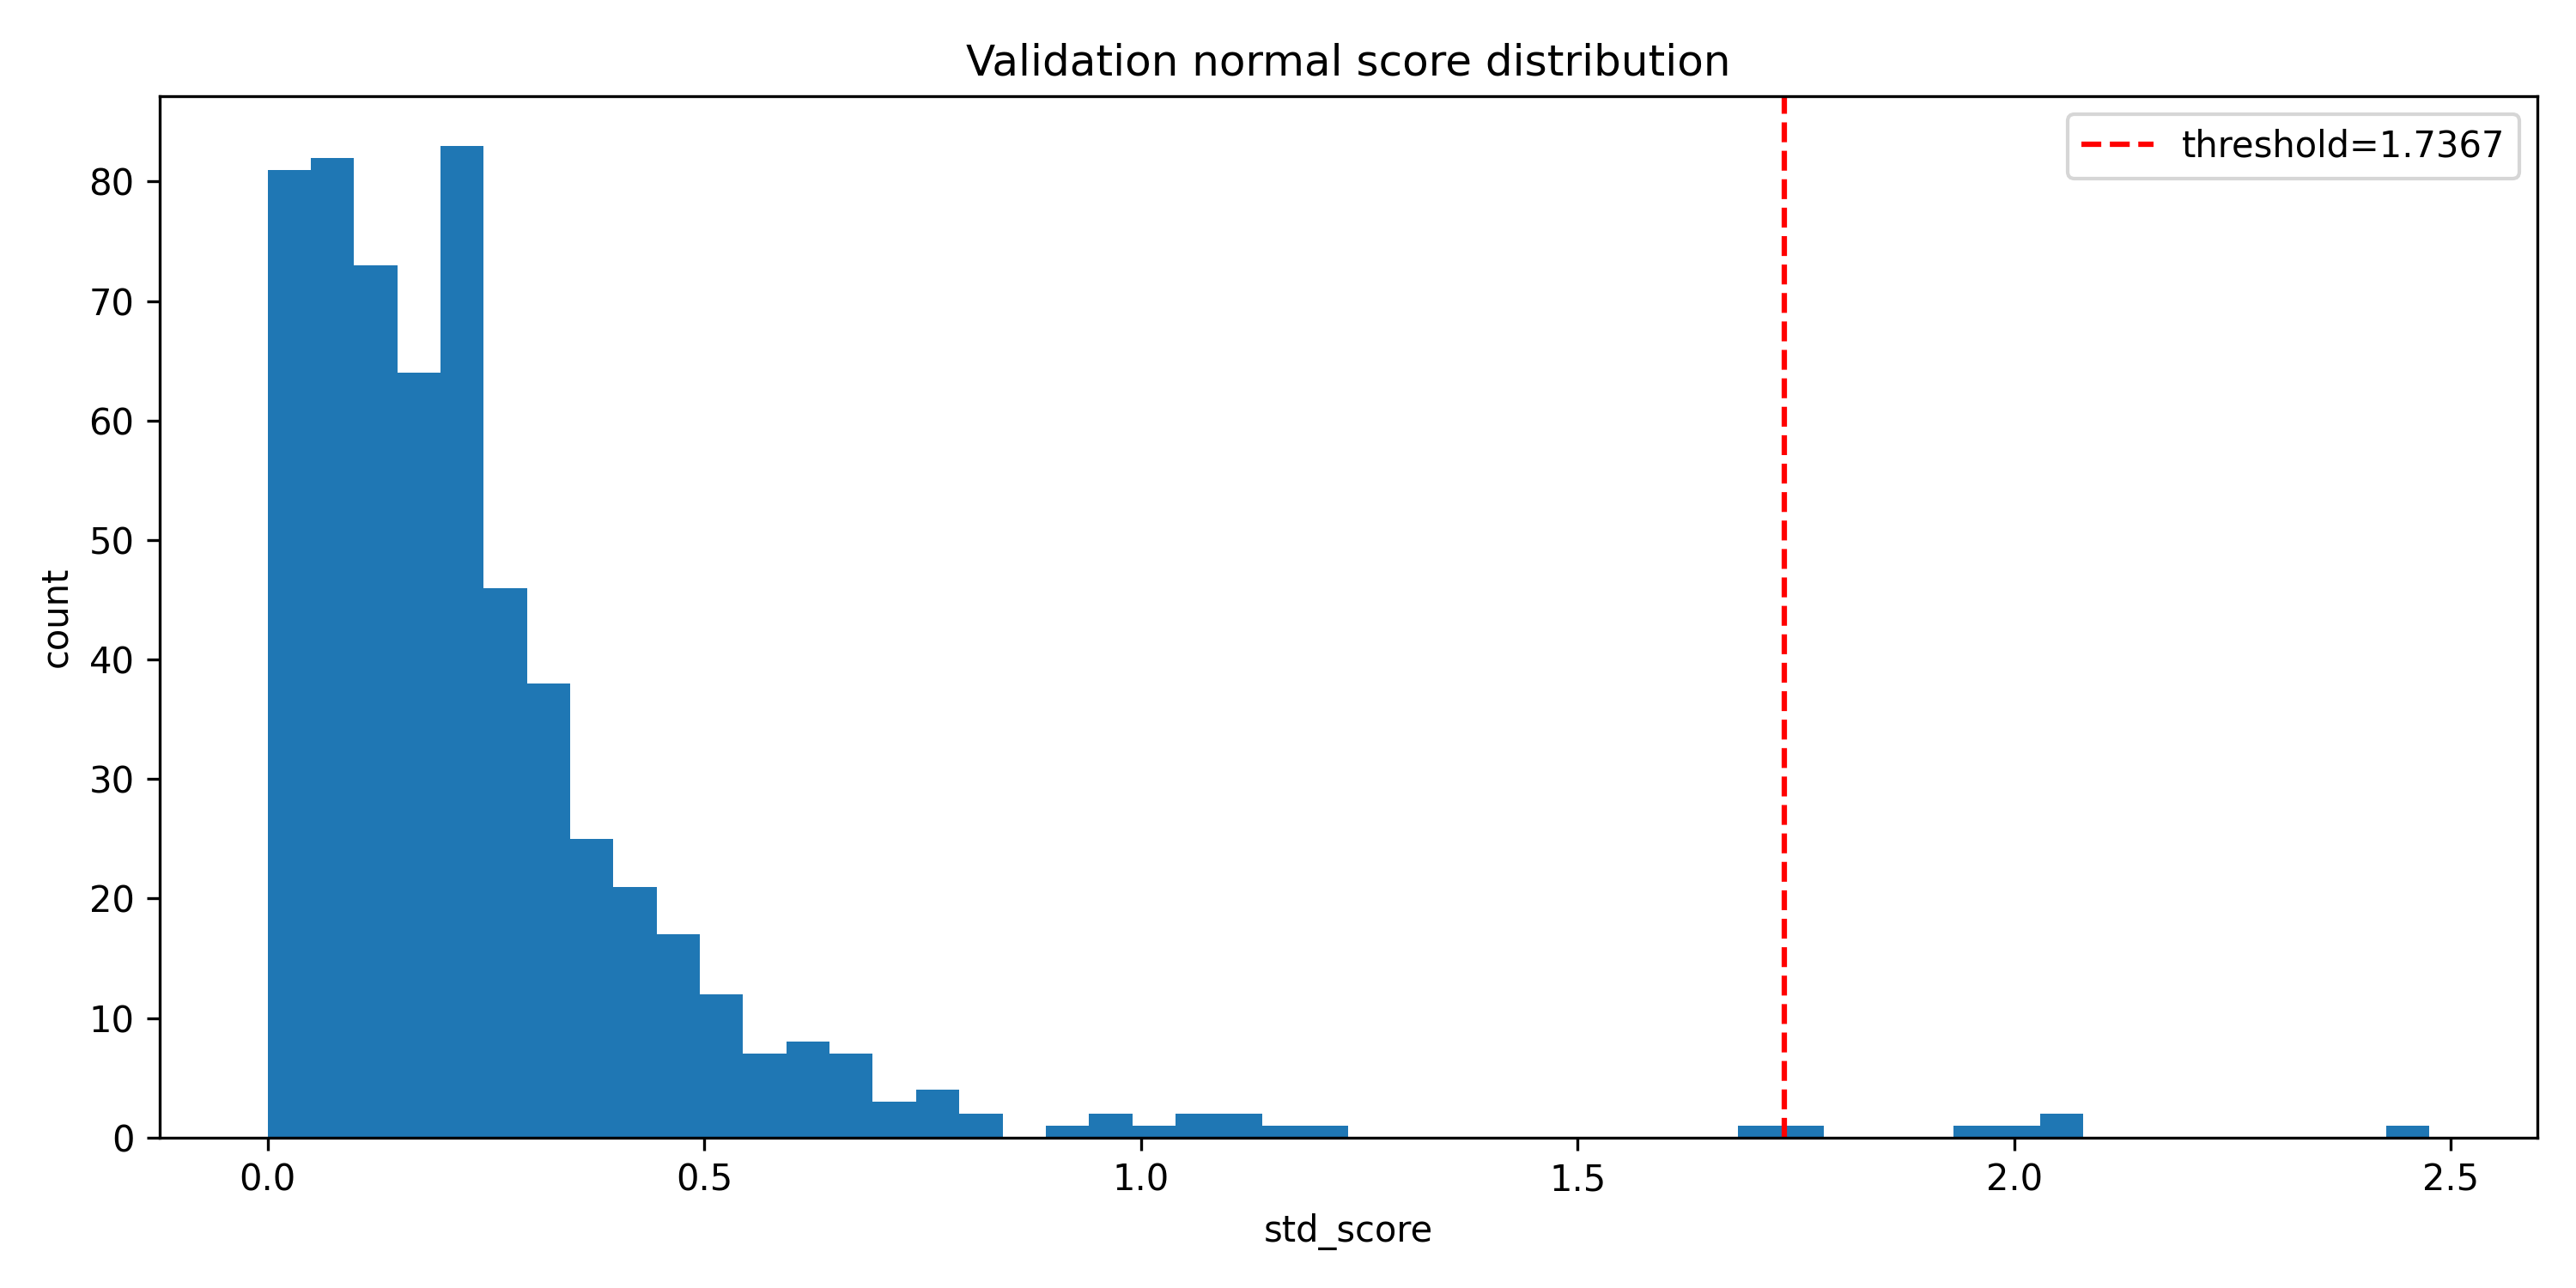
\includegraphics[width=0.86\textwidth]{validation_score_distribution.png}
\caption{Distribution of validation normal anomaly scores with the selected threshold.}
\label{fig:valdist}
\end{figure}

\subsection{Main detection results}

\begin{table}[H]
\caption{Aggregate detection results for final configuration.}
\label{tab:summary}
\centering
\begin{tabular}{lrrrrr}
\toprule
Dataset & Files & Threshold & Precision & Recall & F1-score \\
\midrule
Validation normal & -- & 1.7367 & -- & -- & -- \\
Infected only & 5 & 1.7367 & -- & -- & -- \\
Mixed & 5 & 1.7367 & 1.0000 & 0.9754 & 0.9872 \\
\bottomrule
\end{tabular}
\end{table}

As shown in Table~\ref{tab:summary}, the final detector identifies most mixed infected windows while producing no false positives. The infected-only files are not evaluated with precision and recall because they do not contain normal intervals; instead, their positive window rate is used. The mean infected-only positive window rate is 0.9984, meaning that almost all infected-only windows exceed the anomaly threshold.

\begin{table}[H]
\caption{Per-scenario metrics on mixed normal-infected files.}
\label{tab:mixed}
\centering
\small
\begin{tabular}{lrrrrr}
\toprule
Scenario & Windows & TP & FP & FN & F1-score \\
\midrule
Browser sample 1 & 597 & 202 & 0 & 1 & 0.9975 \\
Generic infected & 572 & 202 & 0 & 1 & 0.9975 \\
Monero sample & 597 & 201 & 0 & 2 & 0.9950 \\
Monero with browser activity & 597 & 202 & 0 & 1 & 0.9975 \\
Stock activity sample 1 & 597 & 183 & 0 & 20 & 0.9482 \\
\bottomrule
\end{tabular}
\end{table}

Table~\ref{tab:mixed} gives the per-file mixed results. The false positive count is zero in every mixed scenario. False negatives are concentrated near scenario boundaries and in the stock-activity sample, while no false positives are observed. The first detected event starts at 1970 seconds in all mixed files, which is 30 seconds before the nominal infected start. This negative delay is explained by the labeling convention: a window can overlap the infected interval before its start timestamp reaches 2000 seconds because the full window span includes both the past input and forecast horizon.

\begin{figure}[H]
\centering
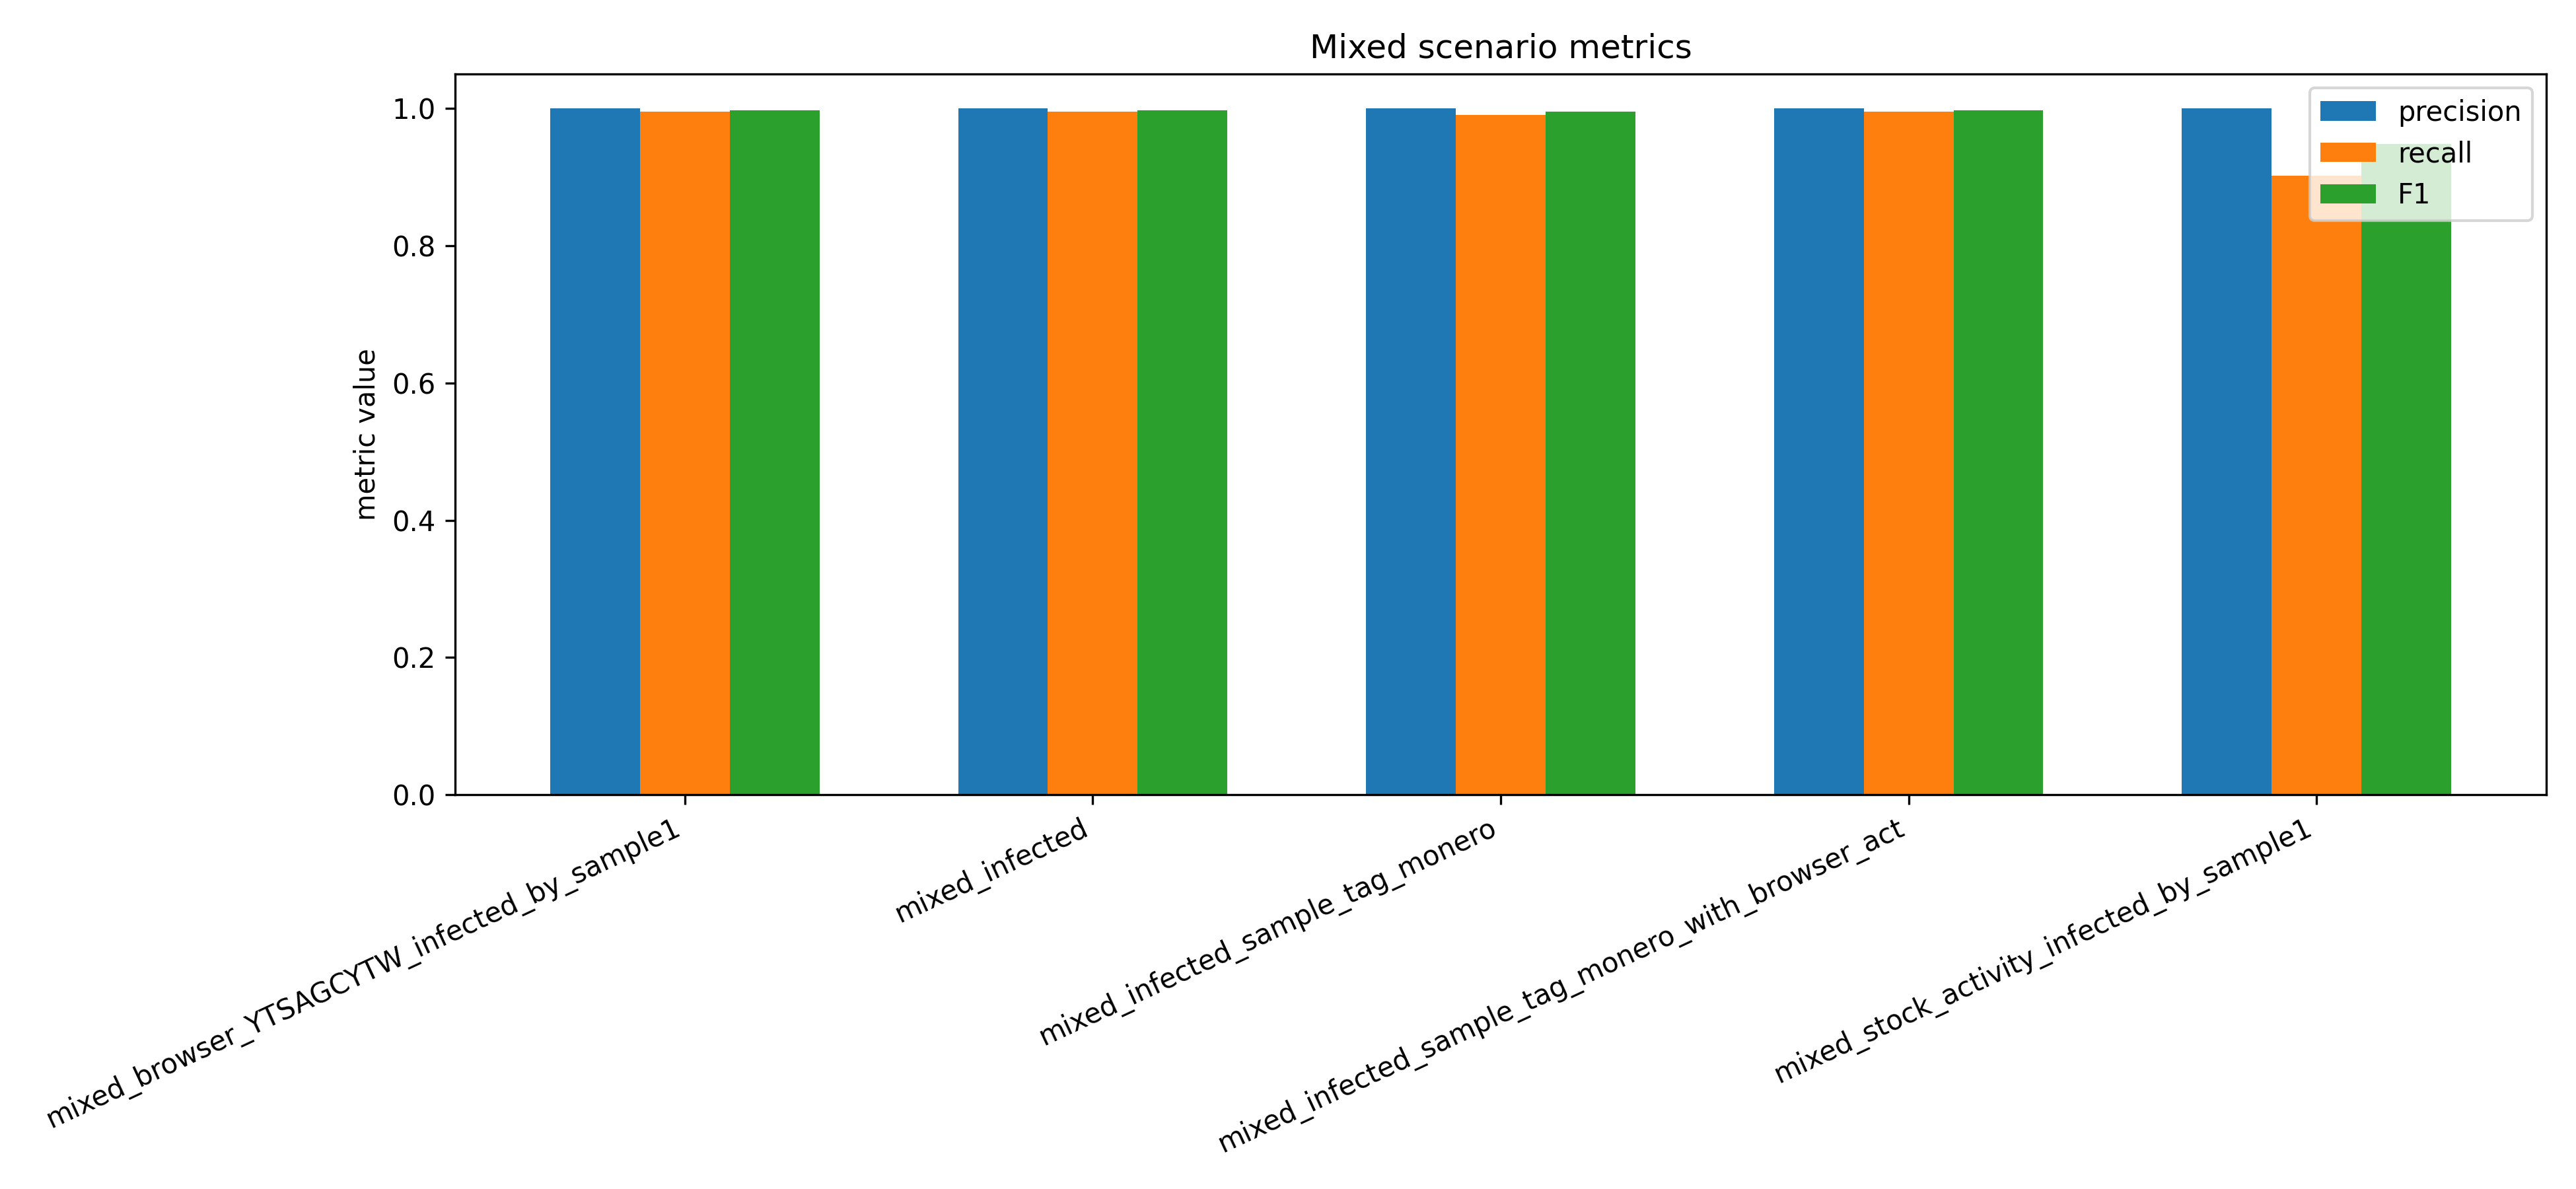
\includegraphics[width=0.95\textwidth]{mixed_metrics_bar.png}
\caption{Precision, recall, and F1-score for mixed scenarios.}
\label{fig:mixedbar}
\end{figure}

Figure~\ref{fig:mixedbar} shows high performance across mixed scenarios, with the stock-activity sample being the most difficult case after GPU features are removed. The total confusion matrix in Figure~\ref{fig:cm} highlights the absence of false positives.

\begin{figure}[H]
\centering
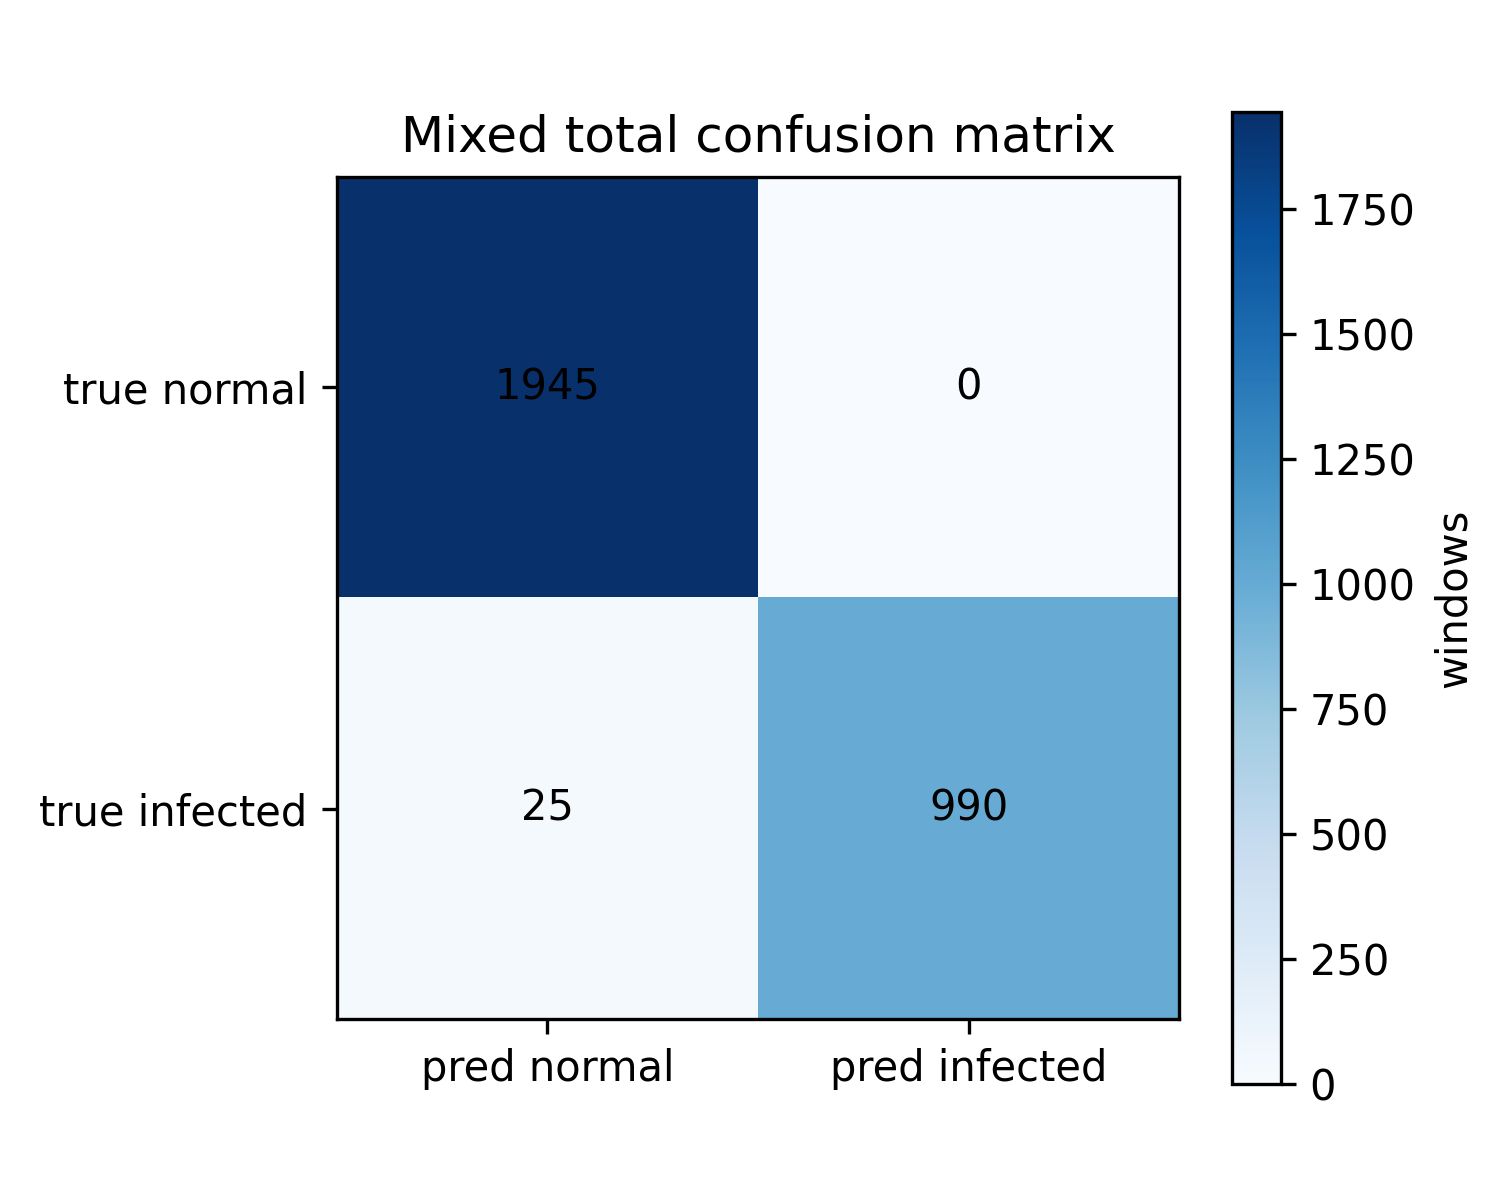
\includegraphics[width=0.56\textwidth]{mixed_confusion_matrix_total.png}
\caption{Total confusion matrix over all mixed scenarios.}
\label{fig:cm}
\end{figure}

\begin{figure}[H]
\centering
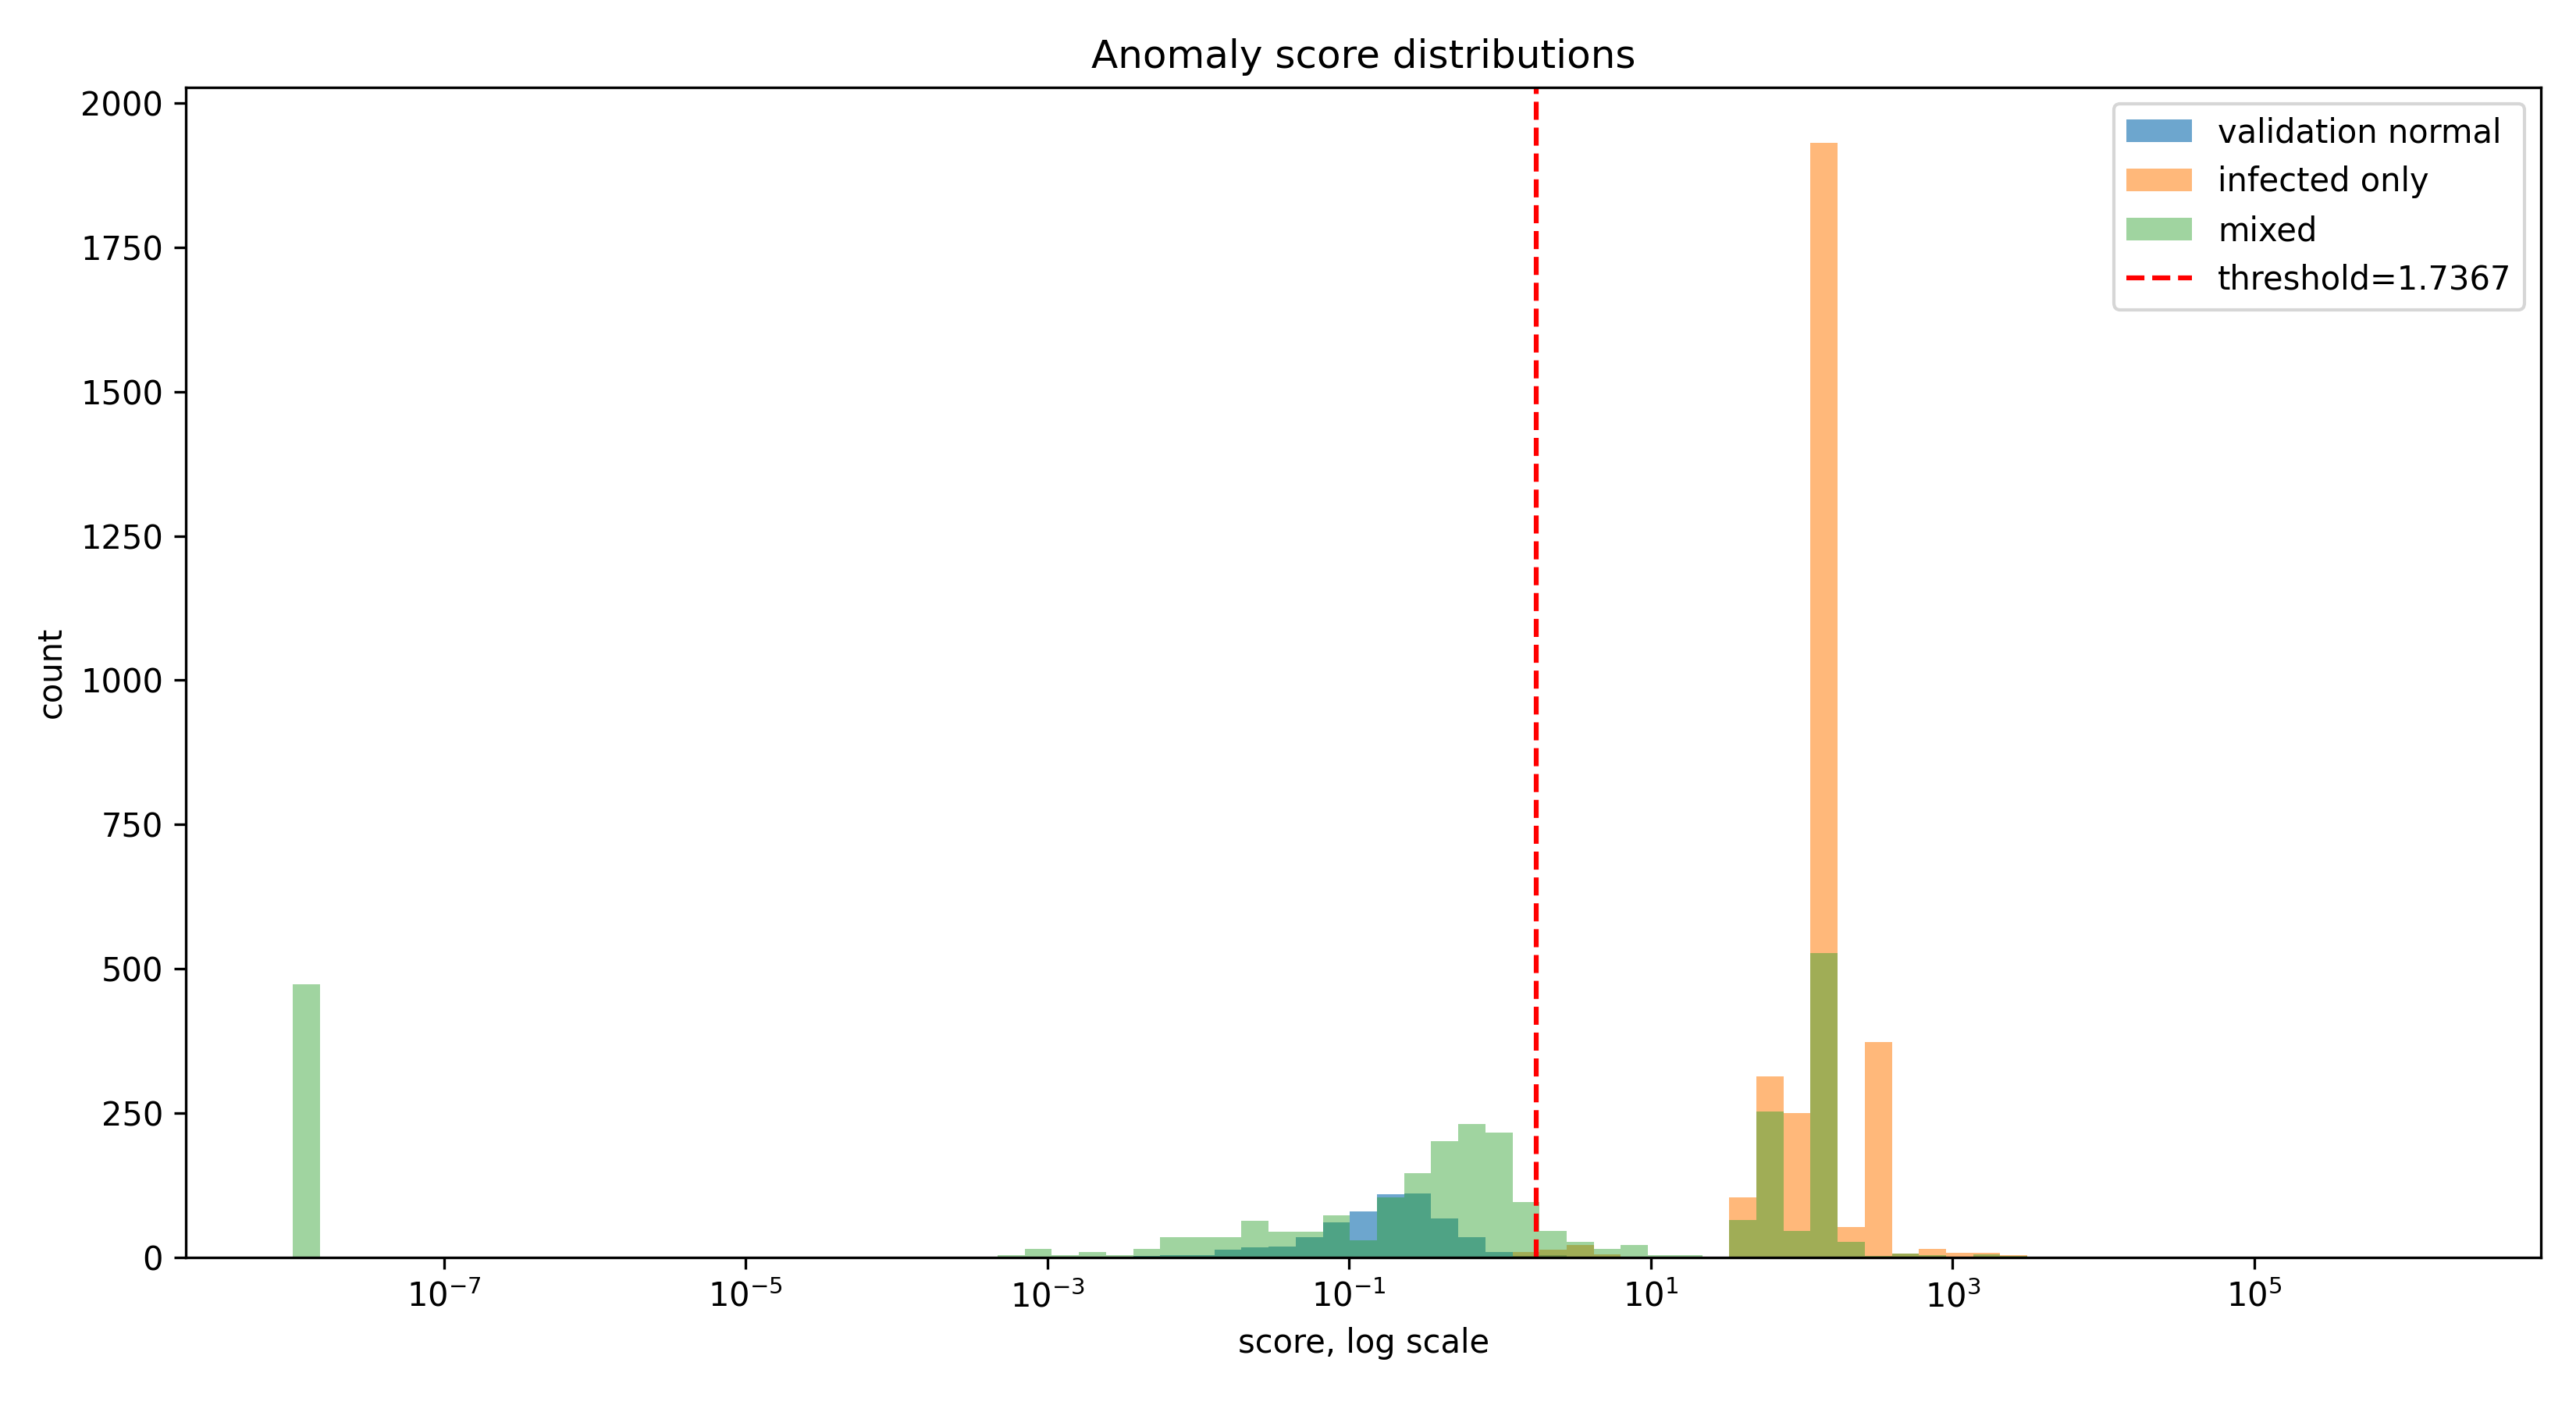
\includegraphics[width=0.95\textwidth]{score_distribution_normal_infected_mixed_log.png}
\caption{Log-scale score distributions for validation normal, infected-only, and mixed data.}
\label{fig:dist}
\end{figure}

Figure~\ref{fig:dist} shows a clear separation between normal validation scores and infected scores. Mixed files contain both normal and infected intervals, so their distribution naturally combines low normal scores and high infected scores.

\begin{figure}[H]
\centering
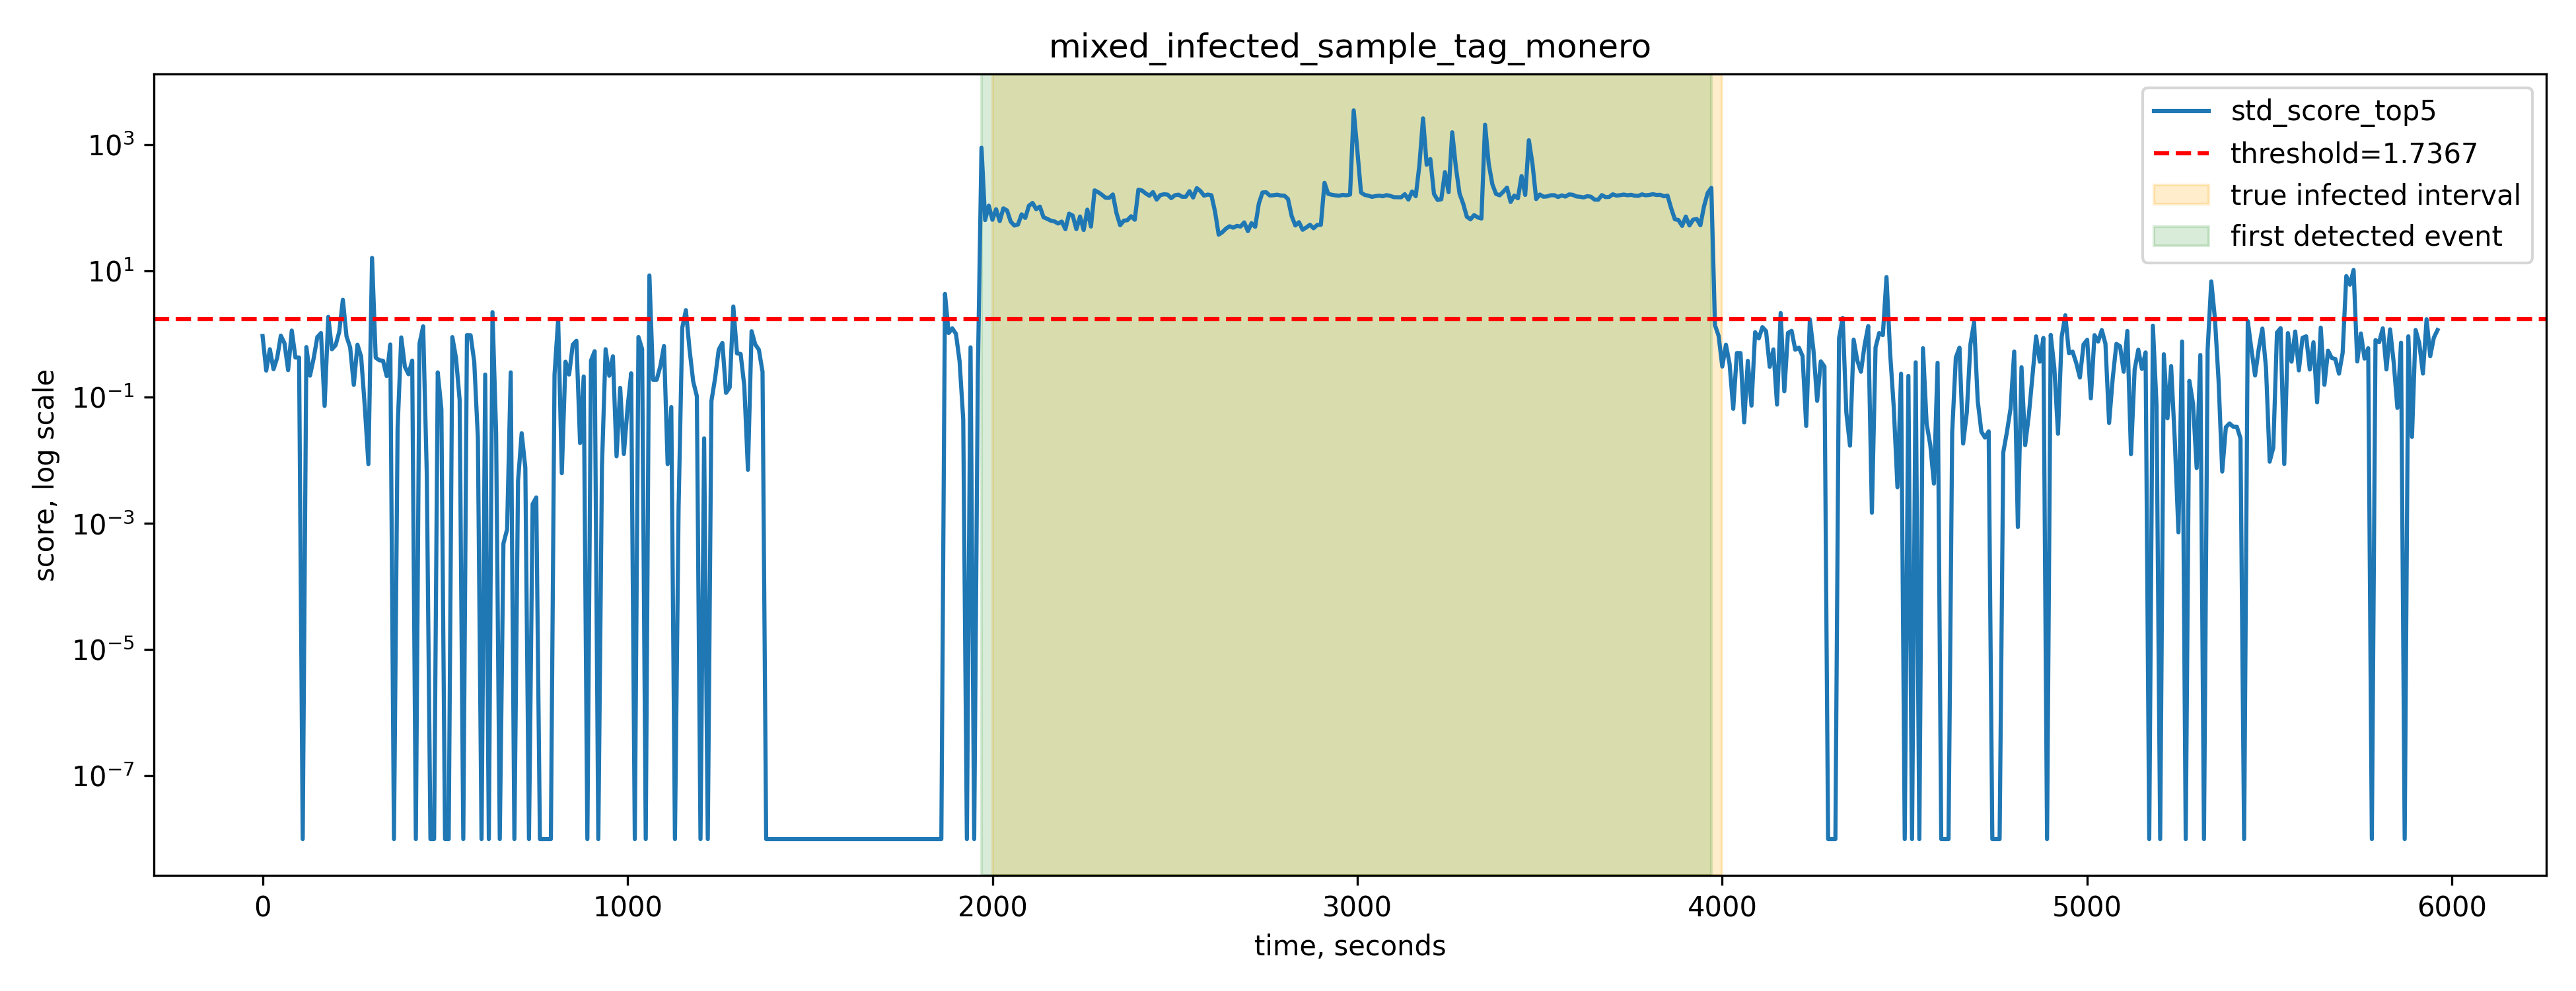
\includegraphics[width=0.95\textwidth]{timeline_telemetry_mixed_normal_infected_sample_tag_monero_normal_clean_1hz.png}
\caption{Representative anomaly-score timeline for a mixed Monero scenario. The orange interval denotes the true infected segment and the dashed line is the threshold.}
\label{fig:timeline}
\end{figure}

The timeline in Figure~\ref{fig:timeline} illustrates the operational behavior of the detector. The score remains below the threshold during normal activity and rises sharply throughout the infected interval.

\subsection{Feature importance}

Feature importance is computed by averaging positive standardized feature errors over selected anomalous windows. This does not provide a causal explanation, but it identifies which telemetry dimensions most strongly contribute to the score.

\begin{table}[H]
\caption{Top feature contributions in mixed positive windows.}
\label{tab:features}
\centering
\begin{tabular}{rlrr}
\toprule
Rank & Feature & Importance share & Windows used \\
\midrule
1 & \texttt{cpu} & 0.4046 & 1082 \\
2 & \texttt{net\_in\_bps} & 0.2660 & 1082 \\
3 & \texttt{p1\_rss\_mb} & 0.0631 & 1082 \\
4 & \texttt{p1\_age\_s} & 0.0560 & 1082 \\
5 & \texttt{net\_out\_bps} & 0.0477 & 1082 \\
\bottomrule
\end{tabular}
\end{table}

Table~\ref{tab:features} and Figure~\ref{fig:featureimp} show that CPU utilization, network input throughput, process memory usage, process age, and network output throughput are the most influential features in the mixed positive windows. This matches the expected behavior of cryptomining activity: sustained computation and resource use are difficult to hide without reducing mining output \cite{darabian2020cryptomining,almurshid2024holistic}.

\begin{figure}[H]
\centering
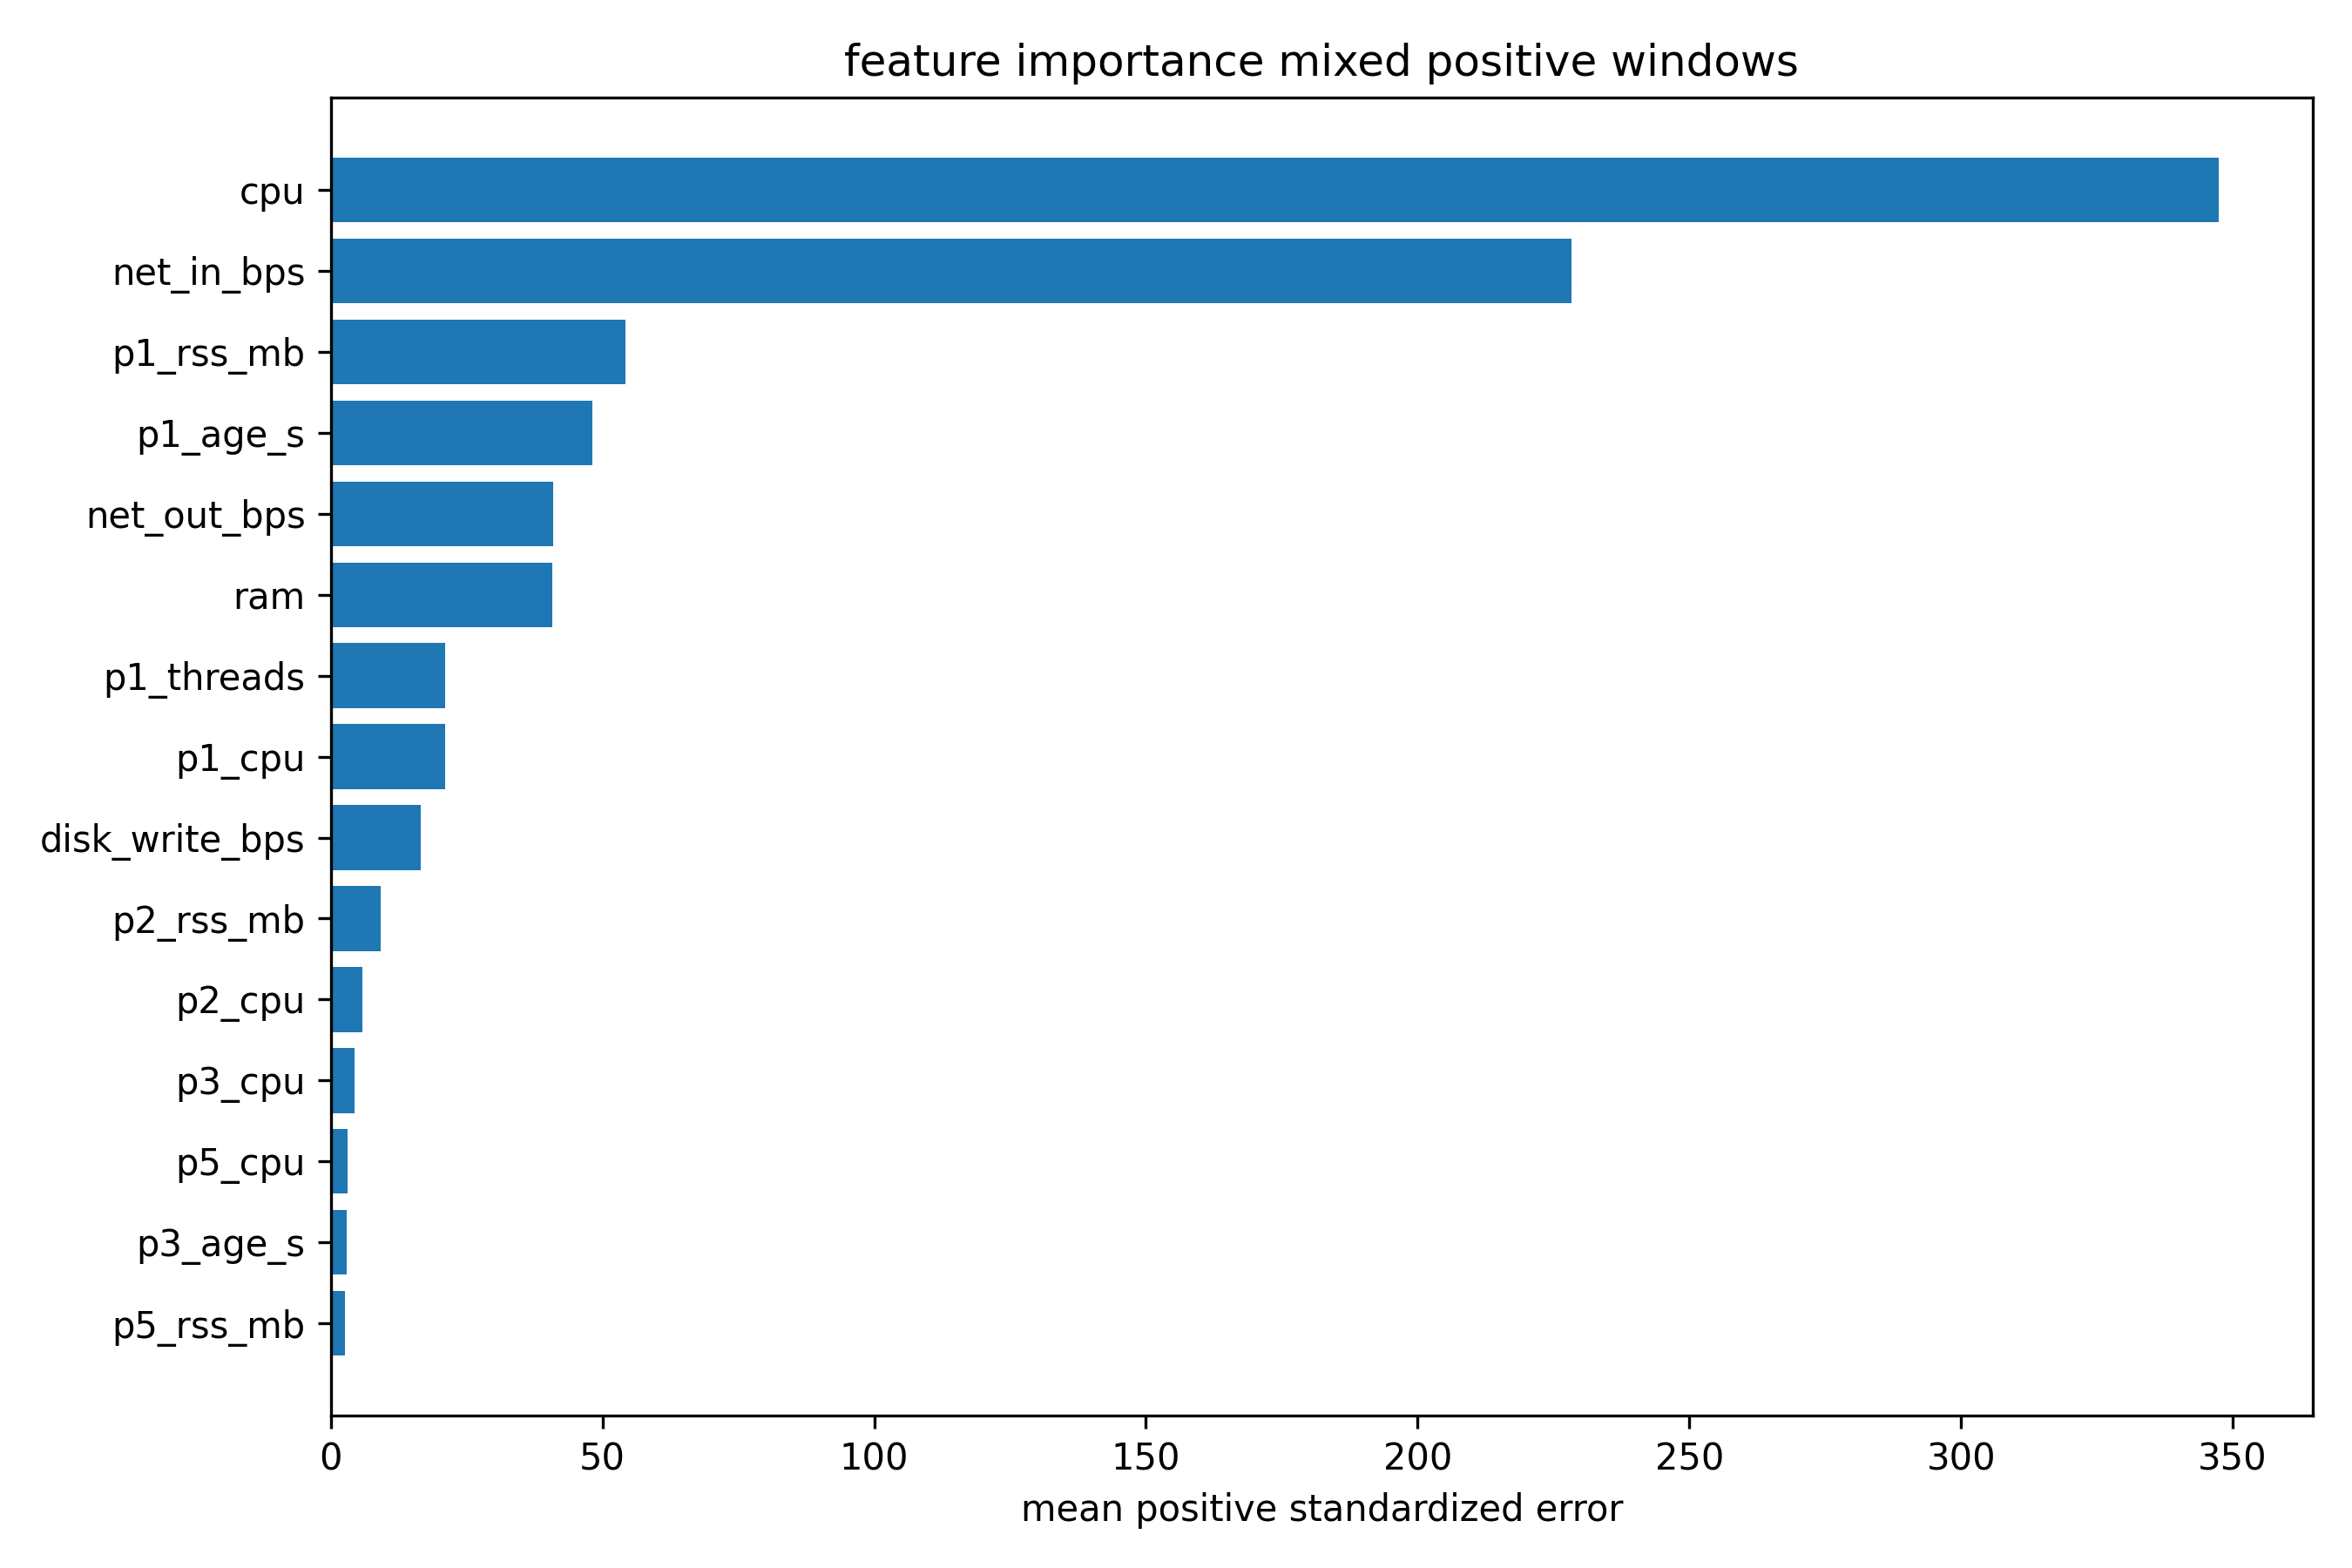
\includegraphics[width=0.82\textwidth]{feature_importance_mixed_positive_windows_top15.png}
\caption{Top 15 feature contributions for mixed positive windows.}
\label{fig:featureimp}
\end{figure}

\subsection{Feature-set correction}

An initial inspection of feature-importance results showed that GPU-related fields received large weights. This was traced to a data-collection limitation: normal telemetry contained real GPU measurements, while infected telemetry contained the same GPU columns filled with constant zeros. Keeping these columns would make the evaluation artificially easier, because the model could learn the missing GPU signal rather than cryptomining behavior.

For this reason, the final experiment excludes all GPU-related columns and retrains the model from scratch. The feature dimensionality decreases from 31 to 26. The resulting metrics are slightly lower than the preliminary full-feature run, but they are methodologically more reliable because the detector now relies on CPU, network, memory, and process-level behavior.

\subsection{Temporal parameter ablation}

Additional experiments were conducted to test the sensitivity of the detector to the input window length $T$ and prediction horizon $H$. In these experiments the same preprocessing and evaluation protocol were used, while one temporal parameter was varied at a time. Each row corresponds to an isolated retrained TCN variant; the final checkpoint reported in the main results is the dedicated final run with the selected $T=30$ and $H=10$ configuration. The purpose was to verify that the chosen final configuration is not an accidental result of a single setting.

\begin{table}[H]
\caption{Ablation over input window length $T$ with $H=10$.}
\label{tab:window_ablation}
\centering
\small
\begin{tabular}{rrrrrr}
\toprule
$T$ & Threshold & Infected rate & Precision & Recall & F1-score \\
\midrule
30 & 1.4751 & 0.9996 & 0.9041 & 0.9931 & 0.9465 \\
60 & 1.3195 & 0.9998 & 0.8846 & 0.9825 & 0.9310 \\
120 & 1.3492 & 0.9998 & 0.8900 & 0.9689 & 0.9277 \\
180 & 1.4040 & 0.9998 & 0.9051 & 0.9358 & 0.9201 \\
240 & 1.3998 & 0.9998 & 0.8971 & 0.9107 & 0.9038 \\
\bottomrule
\end{tabular}
\end{table}

Table~\ref{tab:window_ablation} shows that the shortest tested input window, $T=30$, gives the best mixed-scenario F1-score in this ablation. Longer windows preserve high infected-only positive rates, but recall on mixed scenarios gradually decreases. This supports the final choice of a short context window: cryptomining produces sustained load changes that are visible quickly, and a longer input context may blur event boundaries.

\begin{table}[H]
\caption{Ablation over prediction horizon $H$ with $T=120$.}
\label{tab:horizon_ablation}
\centering
\small
\begin{tabular}{rrrrrr}
\toprule
$H$ & Threshold & Infected rate & Precision & Recall & F1-score \\
\midrule
1 & 1.2506 & 0.9989 & 0.8069 & 0.9575 & 0.8757 \\
5 & 1.2789 & 0.9995 & 0.8699 & 0.9642 & 0.9145 \\
10 & 1.4791 & 0.9996 & 0.9046 & 0.9566 & 0.9298 \\
20 & 1.2135 & 1.0000 & 0.8674 & 0.9643 & 0.9133 \\
30 & 1.2311 & 1.0000 & 0.8726 & 0.9664 & 0.9171 \\
\bottomrule
\end{tabular}
\end{table}

The horizon ablation in Table~\ref{tab:horizon_ablation} indicates that very short prediction horizons are less effective. With $T=120$, the best F1-score is obtained at $H=10$, while longer horizons provide slightly higher recall but lower precision. The final model therefore uses $H=10$ as a compromise between early detection, precision, and stable forecasting.

\subsection{Threshold and event-rule tuning}

The event-level rule was also evaluated with several validation-score quantiles and minimum consecutive anomalous-window counts. With the selected threshold quantile 0.9900 and four consecutive anomalous windows, the detector achieved precision 1.0000, recall 0.9754, F1-score 0.9872, and mean FPR 0.0000. Reducing the event length to three windows increased recall to 0.9813, but also introduced false positives and reduced precision to 0.9881. Therefore, the final configuration uses four consecutive windows as a conservative operating point with no false positives in the main mixed scenarios.

\subsection{Comparison with classical baselines}

To compare the proposed deep learning detector with non-neural anomaly detectors, two classical one-class baselines were trained on normal telemetry windows: Isolation Forest and One-Class SVM. Each baseline used the same cleaned 26-feature set with GPU columns excluded, the same $T=30$ windowing scheme, and the same mixed-scenario labeling convention based on the full $T+H$ window span. The decision threshold for each baseline was selected as the 99th percentile of validation normal scores.

\begin{table}[H]
\caption{Comparison with classical anomaly detection baselines.}
\label{tab:classical_baselines}
\centering
\small
\begin{tabular}{lrrrrrr}
\toprule
Model & $T$ & Infected rate & Precision & Recall & F1-score & FPR \\
\midrule
TCN forecaster & 30 & 0.9984 & 1.0000 & 0.9754 & 0.9872 & 0.0000 \\
Isolation Forest & 30 & 0.5707 & 0.5778 & 0.5537 & 0.5468 & 0.1206 \\
One-Class SVM & 30 & 0.9876 & 0.5391 & 0.9438 & 0.6858 & 0.4178 \\
\bottomrule
\end{tabular}
\end{table}

Table~\ref{tab:classical_baselines} shows that the final TCN forecaster outperforms both classical baselines on the mixed scenarios. Isolation Forest detects only part of the infected interval and produces a noticeable false-positive rate. One-Class SVM reaches high recall, but it marks many normal windows as anomalous, leading to low precision and the highest FPR. In contrast, the TCN forecaster preserves high recall while producing no false positives in the main mixed-scenario evaluation.

\subsection{Stress mixed scenarios}

Finally, stress scenarios were generated by blending infected telemetry with normal background behavior using a mixing coefficient $\alpha$. This experiment evaluates whether detectors remain useful when malicious resource usage is partially hidden. Lower $\alpha$ values represent weaker and more stealthy infected signal.

\begin{table}[H]
\caption{Stress-scenario F1-score under decreasing infected-signal strength.}
\label{tab:stress_scenarios}
\centering
\small
\begin{tabular}{rrrr}
\toprule
$\alpha$ & TCN forecaster & Isolation Forest & One-Class SVM \\
\midrule
1.00 & 0.9619 & 0.7389 & 0.6779 \\
0.75 & 0.9594 & 0.5823 & 0.6437 \\
0.50 & 0.9594 & 0.3859 & 0.5216 \\
0.35 & 0.9594 & 0.1945 & 0.4145 \\
0.25 & 0.9619 & 0.0588 & 0.4271 \\
0.15 & 0.8311 & 0.0200 & 0.3984 \\
0.10 & 0.4861 & 0.0000 & 0.3411 \\
\bottomrule
\end{tabular}
\end{table}

The stress results in Table~\ref{tab:stress_scenarios} provide a more nuanced comparison. The TCN forecaster remains close to F1-score 0.96 for $\alpha \geq 0.25$, while Isolation Forest degrades rapidly as the infected signal weakens. One-Class SVM is more sensitive than Isolation Forest in the low-signal cases, but its high false-positive rate limits precision. At the strongest stealth levels, $\alpha=0.15$ and $\alpha=0.10$, the TCN recall also decreases, showing that sufficiently throttled cryptomining remains difficult to detect from workload telemetry alone.

\section{Discussion}
\label{sec:discussion}

\subsection{Interpretation of Results}

The obtained results indicate that workload telemetry contains enough information to detect the cryptomining activity used in the experiments. The final corrected TCN configuration achieves high recall and zero false positives on the main mixed scenarios after removing GPU-related shortcut features. The most important contributing features are CPU utilization, network throughput, and process-level memory and lifetime statistics, which are consistent with the expected behavior of cryptomining workloads.

The ablation experiments show that the detector is sensitive to temporal design choices. A short input window of 30 seconds gives the best result among the tested window lengths, while prediction horizons around 10--30 seconds perform similarly. Threshold tuning further shows that the event-level decision rule is stable across a reasonable range of validation quantiles and consecutive-window requirements.

The classical-baseline comparison shows the benefit of sequence forecasting in the corrected protocol. Isolation Forest misses many infected windows and still produces false positives. One-Class SVM detects most infected windows, but at the cost of a high false-positive rate. The TCN forecaster gives the best balance on the main mixed scenarios and remains strongest in the stress experiment until the infected signal becomes extremely weak.

\subsection{Limitations}

During the work have been found several limitations. In the beginning of collecting data was collector.py was supposed to collect also GPU telemetry, but it turned out that Oracle VirtualBox does not give access to real graphics card, which lead collector.py to put constant 0 instead of true data, later was decided to put away GPU data from not infected samples too, to exclude chance of learning a shortcut way for moedl. Because of that there is no collected gaming activity in virtual machine.

Infected data collection was limited by open repository of malwarebazaar.com.

\subsection{Future Work}

As a future upgrade for these project can be done several things. Getting access to commercial repositories of viruses and using them  for training and evaluation of the model. Getting access to professional testing machines which are able to provide true telemetry of GPU and collecting new infected data with broader scenarios of use, to cover more ways of user activity. Making desktop app which is going to use that model to provide notifications about possible cryptominer threat on the PC of user. Covering more OS's.

\section{Conclusion}
\label{sec:conclusion}

This course project developed a behavioral cryptominer detector based on system workload telemetry. The detector uses a Temporal Convolutional Network \cite{bai2018tcn} trained on normal data to forecast short-term future workload behavior. Anomalies are detected using standardized feature-wise forecasting errors and an event rule for sustained threshold violations.

The implemented final configuration uses $T=30$, $H=10$, and $S=10$. It was evaluated on five infected-only files and five mixed normal-infected scenarios. The mean infected-only positive window rate was 0.9984. On mixed scenarios, the detector achieved mean precision 1.0000, mean recall 0.9754, mean F1-score 0.9872, and mean FPR 0.0000. The most important features were CPU utilization, network input throughput, process memory usage, process age, and network output throughput.

Additional experiments compared the method with Isolation Forest and One-Class SVM, evaluated temporal-window and prediction-horizon sensitivity, tuned the event threshold, and tested stress scenarios with weakened infected signal. These experiments show that the proposed detector is not only effective in the main setup, but also provides useful robustness under blended normal-infected behavior.

The work satisfies the initial objective: it demonstrates that cryptomining activity can be detected without analyzing executable files or relying on malware signatures \cite{redhu2024deep}. The resulting pipeline is reproducible and generates all report artifacts automatically. 

\newpage
\phantomsection
\addcontentsline{toc}{section}{References}
\nocite{*}
\printbibliography[title={References}]

\end{document}
